\documentclass[12pt,a4paper,final]{article}


\usepackage[left=2cm,right=2cm,top=2cm,bottom=2cm]{geometry}
\usepackage{amssymb}
\usepackage{graphicx}
\usepackage{comment}
\usepackage{amsfonts}
\usepackage{subfig}
\usepackage{enumerate}
\usepackage{graphicx}
\usepackage{multirow}
\usepackage{array}
\usepackage{latexsym}
\usepackage{authblk}
\usepackage{bm}
\usepackage{textcomp}%fixed - problem in listing
%\usepackage{am sfonts}
\usepackage{latexsym}
\usepackage{url}
\usepackage{tikz}
\usepackage{booktabs}
\usepackage{multirow}
\usepackage{rotating}
\usepackage{longtable}
\usepackage{color}
\usepackage{mathrsfs}
\usepackage{tabstackengine}
%\usepackage{lscape}
\usepackage{threeparttable}
\usepackage{xspace}
\usepackage{listings}
\usepackage{float}%fixes floating of float objects
\usepackage{color}%for color code
\usepackage{algorithm}
\usepackage{algpseudocode}
\usepackage{mathtools}          %loads amsmath as well
\DeclarePairedDelimiter\Floor\lfloor\rfloor
\DeclarePairedDelimiter\Ceil\lceil\rceil
%-----------------------------------------------------------------------------------


\definecolor{mygreen}{rgb}{0,0.6,0}
\definecolor{mygray}{rgb}{0.5,0.5,0.5}
\definecolor{mymauve}{rgb}{0.58,0,0.82}

\lstset{ 
  backgroundcolor=\color{white},   % choose the background color; you must add \usepackage{color} or \usepackage{xcolor}; should come as last argument
  basicstyle=\footnotesize,        % the size of the fonts that are used for the code
  breakatwhitespace=false,         % sets if automatic breaks should only happen at whitespace
  breaklines=true,                 % sets automatic line breaking
  captionpos=b,                    % sets the caption-position to bottom
  commentstyle=\color{mygreen},    % comment style
  deletekeywords={...},            % if you want to delete keywords from the given language
  escapeinside={\%*}{*)},          % if you want to add LaTeX within your code
  extendedchars=true,              % lets you use non-ASCII characters; for 8-bits encodings only, does not work with UTF-8
  %firstnumber=1000,                % start line enumeration with line 1000
  frame=single,	                   % adds a frame around the code
  keepspaces=true,                 % keeps spaces in text, useful for keeping indentation of code (possibly needs columns=flexible)
  keywordstyle=\color{blue},       % keyword style
  %language=Octave,                 % the language of the code
  morekeywords={*,...},            % if you want to add more keywords to the set
  numbers=left,                    % where to put the line-numbers; possible values are (none, left, right)
  numbersep=5pt,                   % how far the line-numbers are from the code
  numberstyle=\tiny\color{mygray}, % the style that is used for the line-numbers
  rulecolor=\color{black},         % if not set, the frame-color may be changed on line-breaks within not-black text (e.g. comments (green here))
  showspaces=false,                % show spaces everywhere adding particular underscores; it overrides 'showstringspaces'
  showstringspaces=false,          % underline spaces within strings only
  showtabs=false,                  % show tabs within strings adding particular underscores
  %stepnumber=2,                    % the step between two line-numbers. If it's 1, each line will be numbered
  stringstyle=\color{mymauve},     % string literal style
  tabsize=2,	                   % sets default tabsize to 2 spaces
  %title=\lstname                   % show the filename of files included with \lstinputlisting; also try caption instead of title
 %caption=\lstname
}
%----------------------------------------------------------------------
\usepackage{amsthm}
\newtheorem{theorem}{Theorem}
\newtheorem{corollary}{Corollary}[theorem]
\newtheorem{lemma}[theorem]{Lemma}
\newtheorem*{remark}{Remark}
\theoremstyle{definition}
\newtheorem{definition}{Definition}

%----------------------------------------------------------------------
\DeclarePairedDelimiter{\norm}{\lVert}{\rVert} 

%----------------------------------------------------------------------

\title{\underline{Design and Analysis of Algorithms}}
\author{\underline {Sarbajit Ghosh [CrS1911]}}


\begin{document}
\maketitle



\begin{center}
\textbf{Email: }gsarbajit@gmail.com\\
\textbf{MNo: }8100242571\\
\textbf{Website: }\url{https://github.com/ghosh-sarbajit/algo_end_sem_exam}
\end{center}

\begin{enumerate}

%1
\item
\begin{enumerate}
\item
\textbf{Algorithm for LCM: }
\begin{algorithm}[H]
\caption{LCM(n1,n2)}
\begin{algorithmic}[1]
\State $a \gets n1$
\State $r \gets n2$
\While{$r \neq 0$}
	\State $r \gets a\%b$
	\State $a \gets b$
	\State $b \gets r$
\EndWhile
\State \Return (n1 * n2)/a
\end{algorithmic}
\end{algorithm}

\item
\textbf{Complexity: }Given number is n-bit. So we can input $M=2^n$ as highest number. And off course we have the following relation $n=\log_2 M$. Now let given two numbers as input are $M_1$ and $M_2$. Now if we consider the worst case analysis which occurs for Fibonacci sequence in that case the complexity might be $max\{M_1,M_2\}$ or $\mathcal(O)(M)$. Now to obtain LCM form gcd we are multiplying and dividing two inserted numbers. Hence complexity for calculating multiplication and division is $\mathcal(O)(M_1*M_2)$ or for large numbers approximately $\mathcal(O)(M^2)$.
 

\item
\textbf{C program for LCM: }
\lstinputlisting[language=C]{1c.c}

Here we have used int type variable to store a number, a typical c compiler provides 4 bytes for storing an integer. Now in our algorithm we have to perform multiplication operation. Now for 2 n-bit integer their multiplication value will be upto 2-bit, hence there is a chance of integer overflow. So our program is able to compute LCM of both integers upto $2^16$ if we take unsigned integers off course.

\end{enumerate}


%2
\item
Not attempted.

%3
\item
\begin{enumerate}
\item
\textbf{Mergesort: }
\lstinputlisting[language=C]{3a.c}


\item
\textbf{Program to generate sequence: }
\lstinputlisting[language=C]{3b.c}

\begin{figure}[H]
\includegraphics[width=1.0\textwidth]{3b.png}
\caption{Sorting generated numbers, $x_{-1},x_0,\dots,x_{14}$}
\label{fig:3b}
\end{figure}

\textbf{Explation with $x_1,x_2,\dots,x_{10}$:} 

\begin{figure}[H]
\includegraphics[width=1.0\textwidth]{3b2.JPG}
\caption{Sorting generated numbers, $x_1,x_2,\dots,x_{10}$}
\label{fig:3b2}
\end{figure}
\end{enumerate}


%4
\item
\begin{enumerate}
\item
Here input is a $M_{n \times n}$ matrix.\\
Output is a $N_{n \times n}$ matrix, whose at least one row and and at least one column should be sorted. For row given condition is it should be sorted from left to right in increasing order, while for column it should be sorted  in decreasing order from top to bottom.
\begin{algorithm}[H]
\caption{MatrixSort(M)}
\begin{algorithmic}[1]
\State $r1,r2 \gets Unif\{1:n\}$ \Comment generate two uniform random number from $1,2,\dots,n$
\State $Arr \gets M[r1,]$ \Comment We take $r1^{th}$ row of M
\State $IArr \gets [1:n]$ \Comment An array which contains 1:n
\State OurMergeSort(Arr,IArr) \Comment Internally calls merge sort, rearrange eles of IArr, required to permute cols of $M$
\State $M_1 \gets \,Rearrange(M,IArr,1)$ \Comment 0/1 row/col
\State $Arr \gets M_1[,r2]$
\State $IArr \gets [1:n]$
\State OurMergeSort(Arr,IArr)
\State $M_2 \gets \,Rearranged(M_1,IArr,0)$
\State \Return $M_2$
\end{algorithmic}
\end{algorithm}


%4.b
\item
\textbf{Time complexity: }
\begin{itemize}
\item
For sorting we have $\mathcal{O}(n \log (n))$ comparison in line 4 and 8.
\item
By generating a permutation we are basically creating hash, and Rearrange function with help of that hash value record a particular row of column of its input matrix to its output matrix. So here for recording new elements the complexity is $\mathcal{O}(n^2)$
\item
Hence total time complexity is given by $\mathcal{O}(n^2 + n \log (n))$ which is $\mathcal{O}(n^2)$
\end{itemize}

\textbf{Comment on optimality: }Since all elements here are integer we can use radix sort to get more optimal result.

%4.c
\item
\begin{itemize}
\item
Here we are using array to implement above algorithm.
\item
\textbf{Space complexity: } We are taking two matrix viz $M_1,M_2$, which will comprise of $\mathcal{O}(n^2)$ extra space. And $\mathcal{O}(n)$ amount of extra space for array. So total $\mathcal{O}(n^2)$.
\end{itemize}

\end{enumerate}


%5
\item
\begin{enumerate}
\item

We will present \textbf{Floyed-Warshall} algorithm for all-pair shortest path.\\
Let us consider we have directed weighted graph $(V,E,W)$. Where V, E set of vertex and edges respectively. $W=(w_{ij})$ is adjacency matrix. Let $d^{(k)}_{ij}$ br the weight of shortest path from vertex $i\to j$, for which all intermediate vertices are in $\{1,2,\dots,k\}$. We note that such a path is atleast of length one edge hence,\\
\[
  d^{k}_{ij} =
  \begin{cases}
                      w_{ij}, & \text{if k=0} \\
                      min \{ d^{k-1}_{ij}, d^{k-1}_{ik} + d^{k-1}_{kj} \},  & \text{if k $\geq$ 1}
  \end{cases}
\]
Since for any path, all intermediate vertices are in $\{1,2,\dots,k\}$ and $ d^{k}_{ij} = \delta (i,j), \forall i,j \in V$ at end. We now present the algorithm.

\begin{algorithm}[H]
\caption{Floyed-Warshall(W)}
\begin{algorithmic}[1]
\State $n \gets rows[W]$
\State $D^{(0)}\gets W$
\For{$k\gets 1(1)n$} 
	\For{$i\gets 1(1)n$} 
		  \For{$j\gets 1(1)n$}
		  		 \State $min \{ d^{k-1}_{ij}, d^{k-1}_{ik} + d^{k-1}_{kj} \}$
		  \EndFor 
	\EndFor
\EndFor
\end{algorithmic}
\end{algorithm}

\item
\textbf{Complexity:}In the above algorithm there are 3 loops, each takes $\mathcal{O}(1)$ time to execute hence its complexity is $\mathcal{O}(n^3)$

\item
\end{enumerate}
Here 8 is the number of vertices which is large, so we have write a c program to compute the cost and predecessor matrix.
\textbf{Our  program is as follows :}
\lstinputlisting[language=C]{5c.c}
\textbf{We will use the following adjacent and cost matrix :}

\begin{verbatim}
adjacent matrix
0 1 0 0 1 0 0 0
0 0 1 0 0 1 0 0
0 0 0 1 0 0 0 1
0 0 0 0 0 0 0 0
1 1 0 0 0 0 0 0
0 0 0 0 1 0 0 0
0 0 1 0 0 0 0 0
0 0 1 0 0 0 1 0
cost matrix
0 1 0 4 0 0 0 0
0 0 2 0 0 7 0 0
0 0 0 2 9 0 0 9
0 0 0 0 0 0 0 0
3 5 0 0 0 0 0 0
0 0 0 0 6 0 0 0
0 0 8 0 0 0 0 0
0 0 2 0 0 0 7 0
\end{verbatim}

\textbf{Output is: }
\begin{figure}[H]
\includegraphics[width=1.0\textwidth]{5c.png}
\caption{Floyed-Warshall algo}
\label{fig:5c}
\end{figure}

\textbf{Detailed output we have uploaded: } \url{https://github.com/ghosh-sarbajit}


%6
\item

\begin{enumerate}

\item
\textbf{Largest common subsequence :} Let us consider two sequence of characters $X$ and $Y$. We will say that sequence $Y$ is an subsequence of $X$ if $Y$ can be obtained from $X$ by deleting symbols. \\
\textbf{Example :}Consider $X$=``asdtreerqoplw'' and $Y$=``ateow'', here $Y$ is subsequence of $X$.\\
Now for two strings  $X$ and $Y$ their longest common subsequence will be defined by string $Z$ which can be obtained by omitting symbols from $X$ and $Y$.


\item 
We will solve longest common subsequence problem by using dynamic programming method.\\
Let us consider given strings are $X[1:n]$ and $Y[i:m]$.\\
Let us consider a matrix $A[0:n][0:m]$. In this matrix we will store the the length of longest common subsequence between the two given strings.Based on whether last character of two strings are common or not we can obtain the following recursive relation between elements of $A$.
\[
  A[i][j] =
  \begin{cases}
                      0, & i=0 \lor j=0 \\
                      A[i-1][j-1] + 1,  & X[i]=Y[j],i,j > 0\\
                      max\{A[i-1][j], A[i][j-1]\} & X[i] \neq Y[j],i,j > 0
  \end{cases}
\]

Based on the above algorithm for longest common subsequence is given as follows.
\begin{algorithm}[H]
\caption{Length\_Of\_LCS(X,Y)}
\begin{algorithmic}[1]
\State Initialize A[n+1][m+1]
\State A[0][j]=A[i][0] $\forall i,j \in \{1,\dots,n\} \times \{1,\dots,m\}$
\For{$k\gets 1(1)n$} 
	\For{$i\gets 1(1)m$} 
		  \If{X[i]=Y[j]}
		  		\State A[i][j] $\gets$ A[i-1][j-1] + 1
		  \Else
		  		\State A[i][j] $\gets$ max\{A[i-1][j], A[i][j-1]\}
		  \EndIf
	\EndFor
\EndFor
\State return A
\end{algorithmic}
\end{algorithm}

After finding the length of longest common subsequence we  between we are giving algorithm for finding longest common subsequence string. The following algorithm finds length longest common subsequence with the help of table A.

\begin{algorithm}[H]
\caption{LCS(X,Y,A)}
\begin{algorithmic}[1]
\State Initialize str $\gets \emptyset \land i \gets n \land j \gets m$
\While{$i>0 \land j>0$}
	\If{$X[i]=Y[j]$}
		\State str=X[i] $\circ$ str
		\State i $\gets$ i-1
		\State j $\gets$ j-1
	\ElsIf{A[i][j]=A[i][j-1]}
		\State j $\gets$ j-1
	\Else
		\State i $\gets$ i-1
	\EndIf
\EndWhile
\end{algorithmic}
\end{algorithm}

\textbf{C implementation of above algorithm}
\lstinputlisting[language=C]{6b.c}

\begin{figure}[H]
\includegraphics[width=1.0\textwidth]{6b.png}
\caption{LCS example}
\label{fig:6b}
\end{figure}

\item
\begin{itemize}
\item
Algorithm Length\_Of\_LCS(X,Y) has 2 for loops, and with in each for loop we are doing $\mathcal{O}(1)$ amount calculation hence the complexity is $\mathcal{O}(mn)$.

\item
In algorithm LCS(X,Y,A) the sum m+n is gets decremented, and algorithm stops when it becomes 0. Hence runtime of this algorithm is $\mathcal{O}(m+n)$.
\end{itemize}

\end{enumerate}









%7
\item

\begin{enumerate}
%7.a
\item
A greedy algorithm always makes the choice that looks best at the moment. That is, it makes a locally optimal choice in the hope that this choice will lead to a globally optimal solution. \textbf{-CLRS}\\
\textbf{Example: } An examination system consisting three tier, with the rule that students who had qualified in the first tier are allowed to appear on the second tier and so on, is an example of greedy method of selection.

%7.b
\item
Let, \textbf{G(V,E,W)} be an undirected weighted graph (given). Where V, E, and W are the sets of vertices, edges and edge weights respectively. $W=(w_{ij})$, and $w_{ij}=w(v_i,v_j)$, and $w: E \to \mathbb{R}$\\
\textbf{Minimum Spanning Tree: }A minimum spanning tree (MST) or minimum weight spanning tree is a subset of the edges of a connected, edge-weighted undirected graph that connects all the vertices together, without any cycles and with the minimum possible total edge weight. \textbf{- Wikipedia}\\
We will present \textbf{Kruskal's} algorithm for finding minimum spanning tree. Kruskal algorithm follows greedy approach for finding minimum spanning tree.\\
The algorithm uses disjoint-set data structure.\\
We will use three methods for this data structure, viz. 
\begin{itemize}
\item
\textbf{MakeSet($v_1$): }This method of disjoint-set data structure crates a new set whose only member is $v_1$.
\item
\textbf{Union($v_1,v_2$): }This method of disjoint-set data structure makes union of the dynamic sets containing $v_1, v_2$.
\item
\textbf{FindSet($v_1$): }This method of disjoint-set data structure return a pointer the representative of the dynamic set containing $v_1$.
\end{itemize}


\begin{algorithm}[H]
\caption{$Kruskal(V,E,W)$}
\begin{algorithmic}[1]
\State $T \gets \emptyset$ \Comment An empty set of edges
\For{$\forall v_1 \in V$}
	\State MakeSet($v_1$)
\EndFor
\State sort $e_{ij} \:\forall e_{ij} \in E$ in increasing order of $w_{ij}$ \Comment $e_{ij}$ is edge between $(v_i,v_j), v_i,v_j \in V$
\For{$\forall e_i \in E$ ,taking in increasing order of $w_{ij}$} \Comment \textbf{greedy method used}
	\If{$FindSet(u) \neq FindSet(v)$}
		\State $T \gets T \cup e_{ij}$ \Comment Which is safe for T
		\State Union($v_i,v_j$)
	\EndIf
\EndFor
\State
\Return T
\end{algorithmic}
\end{algorithm}



%7.c
\item
To prove correctness of Kruskal's algorithm we put a \textbf{loop invariant} at the beginning of each loop T should be subset of minimum spanning tree. It works as follows.
\begin{itemize}
\item
\textbf{Initialization: }After initialization T is trivially satisfies \textbf{loop invariant}.
\item
\textbf{Maintenance: } We claim that the procedure follows in for loop of our algorithm, yields a safe edge for T. Also the graph will remain acyclic.
\item
\textbf{Termination: }Since all edges added in the for loop are safe edges, hence our algorithm will return us minimum spanning tree.
\end{itemize}
\textbf{Existence of Safe Edge: }It must exist since $T \subseteq \mathbb{T}$, where $\mathbb{T}$ is minimum spanning tree. Therefore $\exists \, e \in \mathbb{T}\, but \, e \notin T$. Thus $e$ is safe for T. Now correctness of algorithm boils down to finding of an safe edge.\\
Before giving the procedure how find a safe edge and our claim made before we would like to give two definition.\\
\textbf{Cut: } For graph $G=(V,E)$ a cut $(V_1,V-V_1)$ is a partition of $V$. An edge said to be \textbf{crossing the cut} $(V_1,V-V_1)$ if its one end in $V_1$ and other end in $V-V_1$.\\
\textbf{Light edge:} An edge with minimum weight among all the edges which crosses a cut is called light edge.\\
Further a cut $(V_1,V-V_1)$ is said to be \textbf{respect a set} T, if no edges of T crosses the cut.\\ 
Now we shall give a theorem which will establish our claim.\\


\textbf{Theorem: }Let $G=(V,E)$ be a connected, undirected graph a real valued weight function $w: E \to \mathbb{R}$. Let $T \subset E$ and also subset of some minimum spanning tree. Consider $C=(V_C,E_C)$ a connected component in the forest $G_T=(V,T)$, and $e=(v_1,v_2)$ is a light weight edge, which connects $C$ to any other components in $G_T$, then $e$ is safe for $T$.\\
\textbf{Proof: }Given $C$ is a connected component. Hence $(V_C,V-V_C)$ is a cut.\\
Let $\mathbb{T}$ is a MST, which contains $T$. Now if $e \notin \mathbb{T}$ there is no conflict we simply construct $\mathbb{T^\prime}=\mathbb{T}\cup \{e\}$, which will make $e$ safe for $T$, and we are done.\\

Now if $e \in \mathbb{T}$ and its inclusion forms a cycle, with the vertices $v_1 \,and \,v_2 \in T$. Since $e$ belongs to the cut $(V_C,V-V_C)$ therefore $v_1 \in V_C and v_2 \in V-V_C$. Hence there is an edge $\mathbb{T} \ni$ its two vertices are in two sets of cut $C$. Let $e^\prime$ be such an edge. Here we make note that $e^\prime \notin T$ since the cut respects $T$.\\
Now if we remove $e^\prime$ from $\mathbb{T}$ it will break into two components and will again become one if we join them with $e$.\\
Thus we form a new tree as $\mathbb{T^\prime}=\mathbb{T} - e^\prime \cup e$, and by above argument it will be a spanning tree.\\
Now to show that it is also minimum spanning tree, $e$ was the light weight edge that was crossing the cut.\\
Hence, $w(e) \leq w(e^\prime)$.\\
$w(\mathbb{T})=w(\mathbb{T}) - w(e^\prime) + w(e)) \leq w(\mathbb{T})$\\
Again, $w(\mathbb{T}) \leq w(\mathbb{T})$ as $\mathbb{T}$ is a minimum spanning tree.\\
So $\mathbb{T^\prime}$ is also MST. To show that $e$ is safe for $T$ we notice that,\\
$T \subseteq \mathbb{T^\prime}\,and\, T \subseteq \mathbb{T} also \, e^\prime \notin T$. Thus $T \cup e \subseteq T^\prime.$ So $e$ is safe for $T$ this fact follows from $T^\prime$ is also minimum spanning tree.
Hence the result follows.   \textbf{(Proved)}\\
As in each step of the Kruskal algorithm we are including a safe edge each time the set $T$ always remains acyclic. Thus Kruskal algorithm indeed provides a minimum spanning tree.





%7.d
\item
Complexity of Kruskal algorithm on the assumption that it has been implemented using disjoint set forest.
\begin{itemize}
\item
In line 5 there are $\mathcal{O}(|E|log(|E|))$ many operations.
\item
In for loop $\mathcal{O}(|E|)$ many FindSet and Union operation. $\mathcal{O}(|V|)$ many MakeSet operation. Therefore total $\mathcal{O}((|V|+|E|) \alpha(|V|))$ many operations. Where $\alpha(|V|)$ is a small growing function of $|V|$.
\item Hence complexity is $\mathcal{O}(|E|log(|E|))$, or $\mathcal{O}(|E|log(|V|))$. [By remembering $|E| < |V|^2$ ]
\end{itemize}

\end{enumerate}


%8
\item

\begin{enumerate}
%8.a
\item
We will start by giving some necessary definition.
Let $G=(V,E)$ be an directed graph and $c: E \to \mathbb{R}^+$ be a real valued cost function. We choose two $s,t \in V$ as the source and sink vertex.

\textbf{Maximum flow problem: }
\begin{definition}
\textbf{Flow: }A flow is a function $f: E \to \mathbb{R}^+$ with the following constraints\\
1. $\forall\,(v_1,v_2)\in E,\,\, 0\leq f(v_1,v_2) \leq c(v_1,v_2)$ [Known as capacity constraint]\\
2. $\forall\, v \in V - \{s,t\}$
$$\sum_{x \in N_{in}(v)}^{} f(x,v) = \sum_{x \in N_{out}(v)}^{} f(v,y)$$
[Known as conservation constraint]
\end{definition}

Value of the flow is, $$|f| = \sum_{x \in N_{out}(v)}^{} f(v,y) - \sum_{x \in N_{in}(v)}^{} f(x,v)$$ in a network where in source node there are both in and out edges. Max flow problem is to maximize $|f|$.

\textbf{Minimum cut problem: }
\begin{definition}
\textbf{s-t cut: }Here we will partition set $V$ into two sets $S and V \ni \, V = S \cup T$ where $S, T$ are disjoint set of vertices, and $s \in S \land t \in T$. Now cost of cut is defined by $$\norm[\big]{S,T} = \sum_{v_1 \in S,v_2 \in T}^{} c(v_1,v_2)$$.
\end{definition}

\textbf{An Assumption: }We impose a condition on $G$. For $v_1,v_2 \in G.V$ both edges $(v_1,v_2) and (v_2,v_1)$ are not in $E$. If they are we can easily transform the given graph introducing another new vertex $v^\prime$ and edges $(v_1,v^\prime) and (v^\prime,v_1)$.



\begin{definition}
\textbf{Residual capacity: }Here our objective is to improve the flow. In order to that we would like to introduce residual flow as $c_f : V \times V \to \mathbb{R^+}$
\[
  c_f(v_1,v_2) =
  \begin{cases}
                      c(v_1,v_2) - f(v_1,v_2), & if (v_1,v_2) \in E \\
                      f(v_1,v_2),  & if (v_2,v_1) \in E\\
                      0, & else
  \end{cases}
\]
\end{definition}


\begin{definition}
\textbf{Residual graph: }We define $G_f$ to be a residual network wrt. a flow $f$, where $G_f.V=G.V$ and $(v_1,v_2) \in G_F.E$ if $c_f(v_1,v_2) > 0$
\end{definition}

Now we shall give three lemma which will build the very foundation of Ford-Fulkerson’s algorithm for finding the minimum cut which will maximize the flow.

\begin{lemma}
\label{l1}
For many flow $f$ and a cut $(S,T)$ of $G$, we have $|f| \leq \norm[\big] {S,T}$
\end{lemma}


\begin{lemma}
\label{l2}
For a graph $G$ and a given flow $f$, if sink node is not reachable from source node then in its residual graph $G_f$ then flow $f$ is maximum.
\end{lemma}

\begin{lemma}
\label{l3}
For a graph $G$ and a given flow $f$, if sink node is reachable from source node then in its residual graph $G_f$ then flow $f$ is not maximum. Moreover $\exists \, f^\prime$ another flow $\ni$ $|f| \leq |f^\prime|$.
\end{lemma}

We will give the proof Lemma 3, as part of question question 8.c. Now with the above introduced concept we can now present Ford-Fulkerson’s algorithm.

\begin{algorithm}[H]
\caption{$FordFulkerson(G,s,t)$}
\begin{algorithmic}[1]
\State Ini $f \gets 0$
\For{$\forall e \in E$}
	\State $f(e) \gets 0$ \Comment $e=(v_1,v_2)$
\EndFor
\State Run any path finding algorithm to find a path from $p:s  \leadsto t$ in residual graph $G_f$ 
\While{$\exists \, p:s \leadsto t$ in $G_f$}
	\State $c_f(e) \gets min\{c_f(e): \, e \in p\}$
	\For{$\forall \, e \in P$}
		\If{$e=(v_1,v_2 \in E$} \Comment Update flow wrt residual network
			\State $f(v_1,v_2) \gets f(v_1,v_2) + c_f(p)$
		\Else
			\State $f(v_2,v_1) \gets f(v_2,v_1) - c_f(p)$
		\EndIf
	\EndFor
\EndWhile
\State
\Return $f$
\end{algorithmic}
\end{algorithm}


%8.b
\item
Not attempted.

%8.c
\item
Correctness of Ford-Fulkerson theorem follows from Lemma 2 and Lemma 3. Here we will give proof of \textbf{Lemma 3}.
\begin{proof}
Let $p:s \leadsto t$ be a simple path in $G_f$ and $F = min_i \{c(e_i): e_i \in p\}$ and $e_i=(v_1,v_2)$. Based on above we define a new flow as follows,
\[
  f^\prime(v_1,v_2) =
  \begin{cases}
                      f(v_1,v_2) + F, & if (v_1,v_2) \in p \\
                      f(v_1,v_2) - F,  & if (v_2,v_1) \in p\\
                      f(v_1,v_2), & else
  \end{cases}
\]
Now we will show that $f^\prime$ is indeed a flow,to prove \textbf{capacity constraints} are satisfied we notice,
\begin{itemize}
\item
If $(v_1,v_2) \in P$ then $0 \leq f(v_1,v_2) + F \leq f(v_1,v_2) + c_f(v_1,v_2) = f(v_1,v_2) + c(v_1,v_2) - f(v_1,v_2)=c(v_1,v_2)$
\item
if $(v_2,v_1) \in p$ then $f(v_1,v_2) - F \leq f(v_1,v_2) \leq c(v_1,v_2)$ and $f(v_1,v_2) - F \geq f(v_1,v_2) - c_f(v_1,v_2) = 0$
\item
Else flow is from original flow
\end{itemize}
To prove \textbf{conservation constraints} are satisfied,


\begin{itemize}
\item
we recall every simple path $p$, uses 0 or two edges on V. If $p$ uses 0 edges on on $V$ the flow value remains intact while going from $f \to f^\prime$. If p uses two edges of $v \in V$ viz. $(v_1,v) \, and \, (v,v_2)$ which are incident to $v$. Here we consider the following cases [Note that edges appearers in opposite direction in residual network]
\item
If $(v_1,v) \, and \, (v,v_2)$ are both in same direction, both incoming and outgoing flow in $v$ if incremented by $F$.
\item
If $(v_1,v) \, and \, (v,v_2)$ both are in opposite direction , both incoming and outgoing flow in $v$ if decreased by $F$.
\item
If $(v_1,v) \, and \, (v,v_2)$ does not have same direction, then in either cases the flow does not change as $F-F=0$.

\end{itemize}
At the end we notice that in $f^\prime$ we have increased the flow by $F$. Its follows from the fact, for $e \in p$, if $e \in E$ the outward flow increased by $F$, and if $-e \in E$ outward flow decreased by $F$. But again from our definition of residual network $F>0$, hence we get $|f^\prime|>|f|$.
\end{proof}

\textbf{Complexity: }Complexity of the above algorithm is given by $\mathcal{O}(|E||f^\prime|)$

\end{enumerate}




%9
\item
\begin{enumerate}
\item
THe idea of 3SAT and vertex cover problem is as follows:
\begin{definition}
\textbf{3SAT: }Consider three Boolean variable viz. $x,y,z$. We define a \textbf{literal} as a Boolean variable and its negation. We also define a \textbf{clause} as combination of several literals connected with $\lor$, e.g. a clause could be $x\land \bar{y}$. We will say that a clause is in \textbf{conjunctive normal form} or in \textbf{cnf form} if several clause is connected by $\land$.\\
Now we consider a boolean function $\phi$ in three boolean variable which is in \textbf{cnf form} is given  \textbf{3SAT problem} is to check whether there is an combination of $(x,y,x)$ which satisfies to given Boolean function. Since clauses in the Boolean function is connected by $\land$ operator, equivalently we may say that we have to find a combination of $(x,y,x)$ which satisfy all the clauses in the given Boolean function simultaneously.\\
\end{definition}

\begin{definition}
\textbf{Vertex cover problem: }Let us consider an undirected graph $G=(V,E)$. A of $G$ is a set $V^\prime \subseteq V$ such that each edge of $G$ touches one of these nodes. The vertex cover problem, is  given a graph $G$ and a number $k$ whether there is a vertex cover of size $k$ in $G$.
\end{definition}

\item
Here we have to prove the \textbf{vertex cover problem} is \textbf{NP-complete} \textbf{on the assumption that 3SAT problem is NP-complete}. Before giving the proof we would like to give, some definitions.
\begin{definition}
\textbf{NP: }Is the set of languages, whose solution can be guessed, and that guess can be verified by some ``Turin machine" in polynomial time.
\end{definition}

\begin{definition}
\textbf{NP-Hard: }Let $L$ be an given language. $L$ will be NP-Hard if $\forall \, L^\prime \in NP \,\, L^\prime \leq_{P} L$, i.e $L^\prime$ is reducible to $L$ in polynomial time.
\end{definition}

\begin{definition}
\textbf{NP-Complete: }Let $L$ be an given language. We will say that given language is NP-Complete if,
\begin{itemize}
\item
$L \in NP$
\item
$L$ is $NP$ hard.
\end{itemize}
\end{definition}


%9b internal proof begins after some definition
%vertex cover graph
\begin{figure}[H]

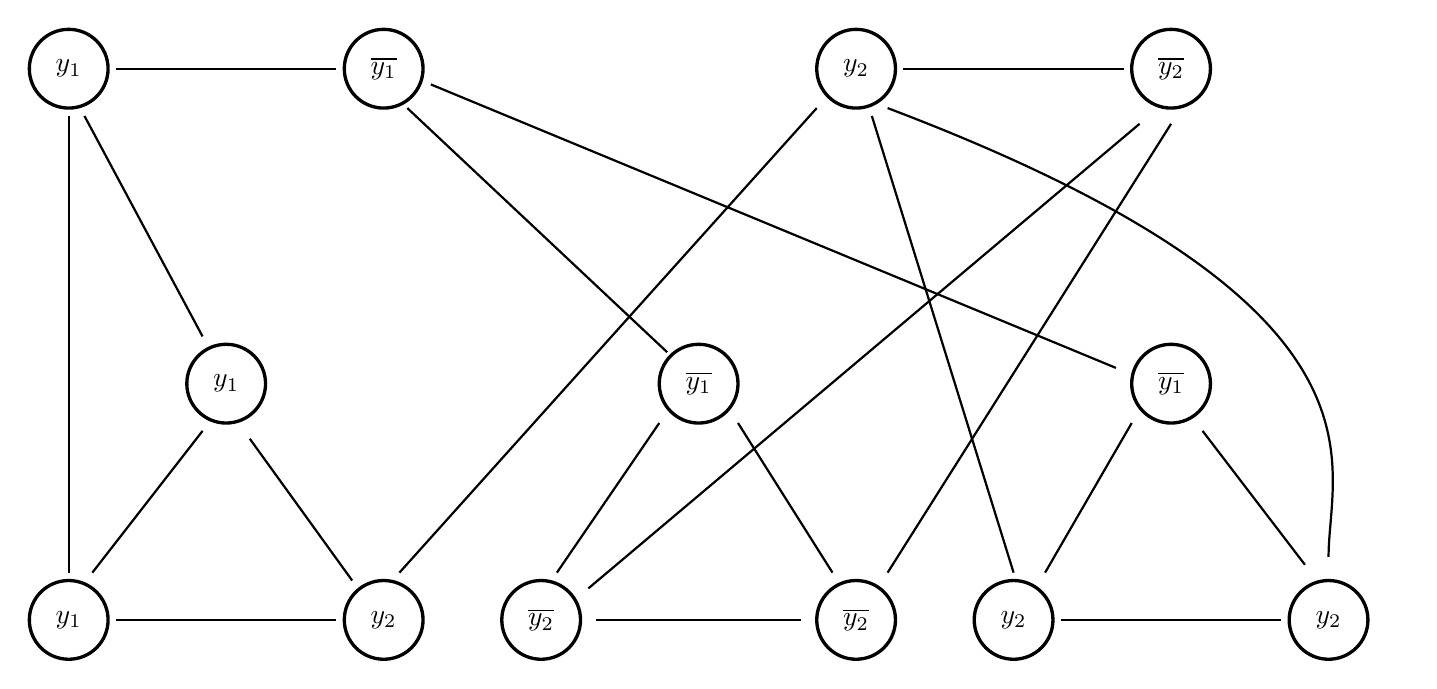
\begin{tikzpicture}

%variable gadget
\draw[very thick](0,0) circle (0.5);
\draw[very thick](4,0) circle (0.5);
\draw[very thick](10,0) circle (0.5);
\draw[very thick](14,0) circle (0.5);


%clause gadget
\draw[very thick](0,-7) circle (0.5);
\draw[very thick](2,-4) circle (0.5);
\draw[very thick](4,-7) circle (0.5);

\draw[very thick](6,-7) circle (0.5);
\draw[very thick](8,-4) circle (0.5);
\draw[very thick](10,-7) circle (0.5);

\draw[very thick](12,-7) circle (0.5);
\draw[very thick](14,-4) circle (0.5);
\draw[very thick](16,-7) circle (0.5);


%names of variable gadget
\draw(0,0) node[anchor=center] {$y_1$};
\draw(4,0) node[anchor=center] {$\overline{y_1}$};
\draw(10,0) node[anchor=center] {$y_2$};
\draw(14,0) node[anchor=center] {$\overline{y_2}$};

%names of clause gadget
\draw(0,-7) node[anchor=center] {$y_1$};
\draw(2,-4) node[anchor=center] {$y_1$};
\draw(4,-7) node[anchor=center] {$y_2$};

\draw(6,-7) node[anchor=center] {$\overline{y_2}$};
\draw(8,-4) node[anchor=center] {$\overline{y_1}$};
\draw(10,-7) node[anchor=center] {$\overline{y_2}$};

\draw(12,-7) node[anchor=center] {$y_2$};
\draw(14,-4) node[anchor=center] {$\overline{y_1}$};
\draw(16,-7) node[anchor=center] {$y_2$};

%Lines
\draw[thick, -] (0.6,0) -- (3.4,0);
\draw[thick, -] (0,-0.6) -- (0,-6.4);
\draw[thick, -] (0.2,-0.6) -- (1.7,-3.4);

%lines(left triangle)
\draw[thick, -] (1.7,-4.6) -- (0.3,-6.4);
\draw[thick, -] (0.6,-7) -- (3.4,-7);
\draw[thick, -] (2.3,-4.7) -- (3.6,-6.5);

\draw[thick, -] (4.3,-0.5) -- (7.6,-3.6);
\draw[thick, -] (4.6,-0.2) -- (13.3,-3.8);
\draw[thick, -] (9.5,-0.5) -- (4.2,-6.4);
\draw[thick, -] (13.6,-0.7) -- (6.6,-6.6);
\draw[thick, -] (14,-0.7) -- (10.4,-6.4);

\draw[thick, -] (10.6,0) -- (13.4,0);

\draw[thick, -] (10.2,-0.6) -- (12,-6.4);
\draw[thick, -] (10.4,-0.5) ..controls (17,-3) and (16,-5).. (16,-6.2);
%\draw (-2,2) .. controls (-1,0) and (1,0) .. (2,2);


%lines(mid triangle)
\draw[thick, -] (7.5,-4.5) -- (6.2,-6.4);
\draw[thick, -] (8.5,-4.5) -- (9.7,-6.4);
\draw[thick, -] (6.7,-7) -- (9.3,-7);

%lines(right triangle)
\draw[thick, -] (14.4,-4.6) -- (15.7,-6.3);
\draw[thick, -] (13.5,-4.5) -- (12.4,-6.4);
\draw[thick, -] (12.6,-7) -- (15.4,-7);


\end{tikzpicture}


\caption{Vertex cover is NP-Complete}
\label{fig:9b}
\end{figure}




\textbf{Now we will move on to the proof}
\begin{proof}
Consider $G$ an undirected graph. $k$ is a given positive integer. Let us define the set, $$VCOV = \{<G,k>|\,undirected\,\, graph\, \,G \,\,has\,\, a\,\, k\,\, many\,\, node\,\, vertex \,\,cover\}$$.
Proving \textbf{vertex cover} is in NP is easy. As a vertex cover of size k will work as certificate.\\

To prove it is NP-hard we will show a map reduction from \textbf{3SAT} to \textbf{Vertex cover}. The reduction focuses on converting a 3cnf formula into a graph and an inter G and k respectively, in such a way that whenever there is a vertex cover of k in G the 3cnf Boolean formula will be satisfied.\\

Let us consider following Boolean function,\\
$$\psi = (y_1 \lor y_1 \lor y_2) \land (\bar{y_1} \lor \bar{y_2} \lor \bar{y_2}) \land (\bar{y_1} \lor y_2 \lor y_2)$$.

Now we set-up \textbf{gadget for variable} as follows for each variable y in $\psi$ we draw two edges into gadget. We level the two nodes in this gadget as $y$ and $\bar{y}$. If the node is included in vertex cover $y$ will be TRUE else FALSE.

To set-up \textbf{gadget for  clause} we do as follows. We combine three interconnected nodes to make a gadget, and connect to \textbf{variable gadget} whenever the label matches.\\

Now if $\psi$ be an $\delta$ variable $\lambda$ clause Boolean function then, total number of nodes in our constructed graph will be $2\delta+3\lambda$. $$Let,\,\, k:=2\delta+3\lambda$$.
Now we will show that our given reduction works,\\
For that we assume that $\psi$ is satisfiable, so we put the nodes of \textbf{variable gadget } corresponding to the true literals in assigned vertex cover and we put one true literal from every clause gadget into vertex cover. This makes cardinality of our vertex cover precisely $k$.\\
Hence 3SAT satisfiability $\implies$ Vertex Cover.\\
Again on the contrary we assume that $G$ has a vertex cover of size $k$. Now this cover must contain one node from every \textbf{variable gadget} and two from every \textbf{clause gadget}, as it has to cover our graph both consisting of both type of gadgets. In order to make $\psi$ satisfiable we assign TRUE to the corresponding literals.\\
Hence Vertex Cover $\implies$ 3SAT satisfiability.\\
This completes the proof.

\end{proof}

\item
Not attempted
\end{enumerate}
















\end{enumerate}
\end{document}
